\documentclass[11pt,paper=letter]{scrartcl}
\usepackage[alttitle]{cjquines}

\setlength{\oddsidemargin}{0.8in}
\setlength{\evensidemargin}{0.9in}
\setlength{\textwidth}{6.8in}
\setlength{\textheight}{8.5in}
\setlength{\headheight}{0pt}
\setlength{\headsep}{15pt}

\pretitle{\vspace{-6em} \begin{flushleft} \bfseries \Large}
\posttitle{\vspace{-0.6em} \end{flushleft}}
\preauthor{\begin{flushleft} \itshape \Large}
\postauthor{\vspace{-0.7em} \end{flushleft}}
\predate{\begin{flushleft} \Large}
\postdate{\end{flushleft} \rule{\textwidth}{0.5pt}}

\begin{document}

\title{$\qquad\qquad\qquad$ Program for Inducing Mathematical Excellence}
\author{$\qquad\qquad\qquad\;\;\,$ Final Exam}
\date{$\qquad\qquad\qquad\quad$ 27 October 2017}

\maketitle
\setlength{\unitlength}{1in}
\begin{picture}(0,0)
  \put(0.1,0.6){\hbox{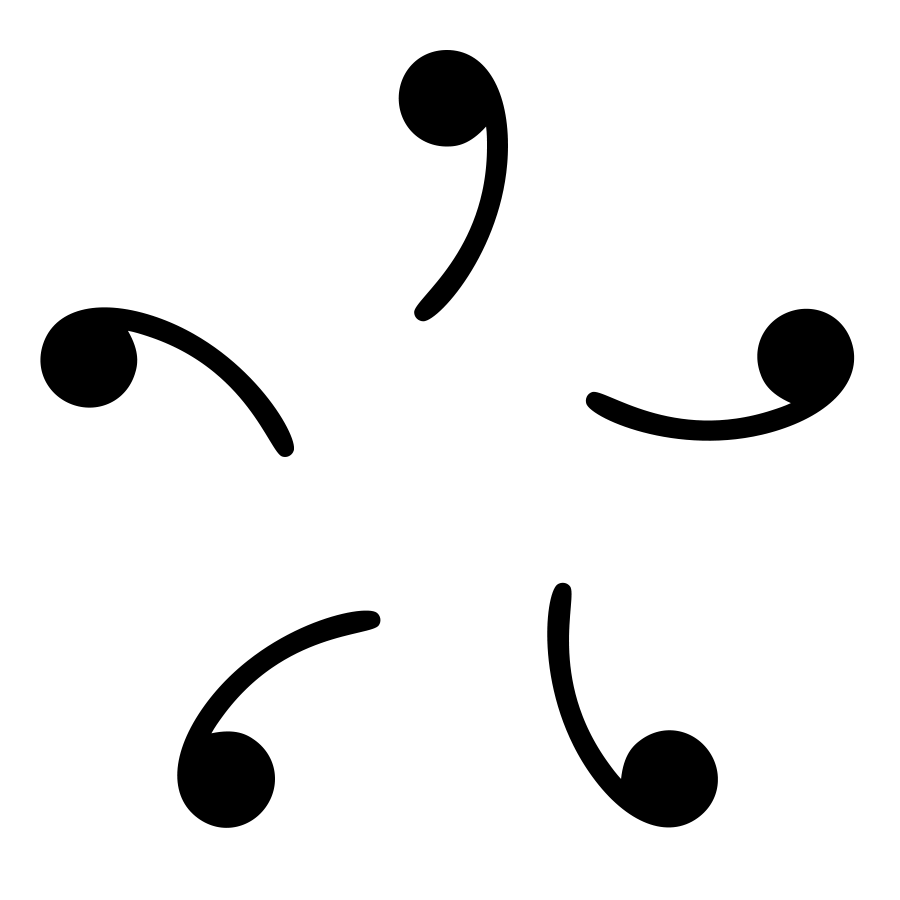
\includegraphics[width=0.9in]{logo.png}}}
\end{picture}
\vspace{-2em}

\noindent\textbf{PART I.} Choose the best answer. Each correct answer is worth two points.

\begin{enumerate}
  \item Which of the following choices is the largest?

  \fourch
  {$121^6$}
  {$12^{12}$}
  {$5^{18}$}
  {$2^{42}$}

  \item In triangle $ABC$, $AB = 6$ and $BC = CA = 5$. Which of the following statements are false?
  \begin{enumerate}
    \item[(a)] Triangle $ABC$ is acute, but if $AB = 8$ instead, it would be obtuse.
    \item[(b)] Of the triangle's angles, the one with the largest measure is $\angle BCA$.
    \item[(c)] The value of $\tan \angle ABC$ is greater than $1.5$ but less than $2$.
    \item[(d)] The area of triangle $ABC$ is numerically equal to three-fourth its perimeter.
  \end{enumerate}
  \vspace{0.5em}

  \item Ankan flips six fair coins. What is the probability he gets more than three heads?

  \fourch
  {$\dfrac{11}{32}$}
  {$\dfrac12$}
  {$\dfrac{21}{32}$}
  {$\dfrac{13}{16}$}

  \item Each of $6$ people picks another person among them as their giftee, and no two people pick the same giftee. Everyone holds a nametag with their name on it. In a single move, each person gives the nametag they're holding to their giftee. After several moves, everyone holds their own nametag again. What is the minimum number of moves needed to ensure this?

  \fourch
  {$12$}
  {$60$}
  {$120$}
  {$144$}

  \item Points $I, A,$ and $N$ are outside regular octagon $PROBLEMS$ such that $PIANO$ is a regular pentagon. What is $m\angle ROA$?

  \fourch
  {$49.5\dg$}
  {$51\dg$}
  {$52.5\dg$}
  {$54\dg$}

  \item John is answering a question on his exam: ``What interval is $50\%$ to $65\%$ of the maximum heart rate of a $20$-year-old?'' John is given the following choices, and he knows the correct answer is one of these. Which of these is the correct answer?

  \fourch
  {$\sbr{100, 130}$ bpm}
  {$\sbr{110, 140}$ bpm}
  {$\sbr{120, 150}$ bpm}
  {$\sbr{130, 160}$ bpm}

  \item Given that $\sin x + \cos x = \dfrac43$, what is the value of $\sin^3 x + \cos^3 x$?

  \fourch
  {$\dfrac{29}{54}$}
  {$\dfrac{17}{27}$}
  {$\dfrac{13}{18}$}
  {$\dfrac{22}{27}$}

  \item Class A has $a$ boys and $b$ girls, while Class B has $x$ boys and $y$ girls, where $a, b, x$ and $y$ are integers such that $0 < a < x < b < y$. Each pupil in Class A is paired with someone from Class B. No pupil is in two different pairs. What is the maximum number of pairs with one boy and one girl?

  \fourch
  {$a+x$}
  {$x+b$}
  {$b+y$}
  {$y+a$}

  \item Suppose the roots of $x^3 + 20x + 17 = 0$ are $a, b$ and $c$. What is $a^3 + b^3 + c^3$?

  \fourch
  {$-34$}
  {$-37$}
  {$-40$}
  {$-51$}
\end{enumerate}

\noindent
\begin{minipage}{0.7\textwidth}
  \begin{enumerate}
    \item[10.] In the figure on the right (not drawn to scale), four gears are shown, represented as circles. Gear $A$ has radius $6$, gear $B$ has diameter $6$, gear $C$ has circumference $6$, and gear $D$ has area $6$. The first gear is turned $90\dg$. By how many radians does gear $D$ turn?

    \fourch
    {$\dfrac{\pi^2}2$}
    {$\dfrac{\pi\sqrt{6\pi}}2$}
    {$\dfrac{\pi^2}4$}
    {$\dfrac{\pi\sqrt{6\pi}}4$}
  \end{enumerate}
\end{minipage}%
\begin{minipage}{0.3\textwidth}
  \begin{center}
    
\includegraphics[width=\textwidth]{f1.png}
  \end{center}
\end{minipage}

\begin{enumerate}[start=11]
  \item Given that $a, b$ and $c$ are positive real numbers satisfying
  \begin{align*}
    ab + 2a + b &= 13,\\
    bc + 3b + 2c &= 36,\\
    ca + c + 3a &= 32,
  \end{align*}
  then $a$ can be written as $\dfrac{p + q\sqrt{r}}s$ for some integers $p, q, r$ and $s$, where $r$ is not divisible by the square of a prime and $p$, $q$ and $s$ have greatest common divisor $1$. What is $p + q + r + s$?

  \fourch
  {$5$}
  {$7$}
  {$9$}
  {$11$}

  \item Each vertex of a regular pentagon is colored either pink, red, indigo, mauve or ebony. Two colorings are the same if one can be rotated to obtain the other. Find the number of different colorings.

  \fourch
  {$5^4 - 1$}
  {$5^4$}
  {$5^4 + 4$}
  {$5^4 + 5$}

  \item Which of the following choices is nearest to $\sqrt{3} + \sqrt{8} + \sqrt{15} + \sqrt{24} + \sqrt{35} + \sqrt{48}$?

  \fourch
  {$26.2$}
  {$26.4$}
  {$26.6$}
  {$26.8$}

  \item Five husbands and their five wives sit in a row. Exactly four wives are sitting next to their respective husbands. In how many ways is this possible?

  \fourch
  {$40\,320$}
  {$44\,160$}
  {$80\,640$}
  {$84\,480$}

  \item What is the remainder when $20^{17} + 17^{20}$ is divided by $21$?

  \fourch
  {$3$}
  {$5$}
  {$15$}
  {$17$}
\end{enumerate}

\vspace{1em}
\noindent\textbf{PART II.} Choose the best answer. Each correct answer is worth three points.

\begin{enumerate}
  \item There exists distinct nonzero digits $a$, $b$ and $c$ such that the eight-digit number $\seg{aaabbbb5}$ is the square of the four-digit number $\seg{ccc5}$. There are two possible values for $a$. What is their sum?

  \fourch
  {$5$}
  {$9$}
  {$13$}
  {$17$}
\end{enumerate}

\noindent
\begin{minipage}{0.75\textwidth}
  \begin{enumerate}
    \item[2.] In the figure on the right, $OA_0 = OA_1 = 1$, and $\angle A_0OA_1 = 90\dg$. First, Bobby draws a circle tangent to $OA_0$ at $A_0$ and to $OA_1$ at $A_1$. For each positive integer $n$, Bobby then draws:
    \begin{enumerate}
       \item a ray $OA_{n+1}$ such that $2\angle A_nOA_{n+1} = \angle A_{n-1}OA_n$, and
       \item a circle tangent to $OA_n$ at $A_n$ and to $OA_{n+1}$ at $A_{n+1}$.
    \end{enumerate}
    Which of the following choices is closest to the sum of the areas of the infinitely many circles Bobby draws?

  \fourch
  {$1.17\pi$}
  {$1.23\pi$}
  {$1.29\pi$}
  {$1.35\pi$}
  \end{enumerate}
\end{minipage}%
\begin{minipage}{0.25\textwidth}
  \begin{center}
    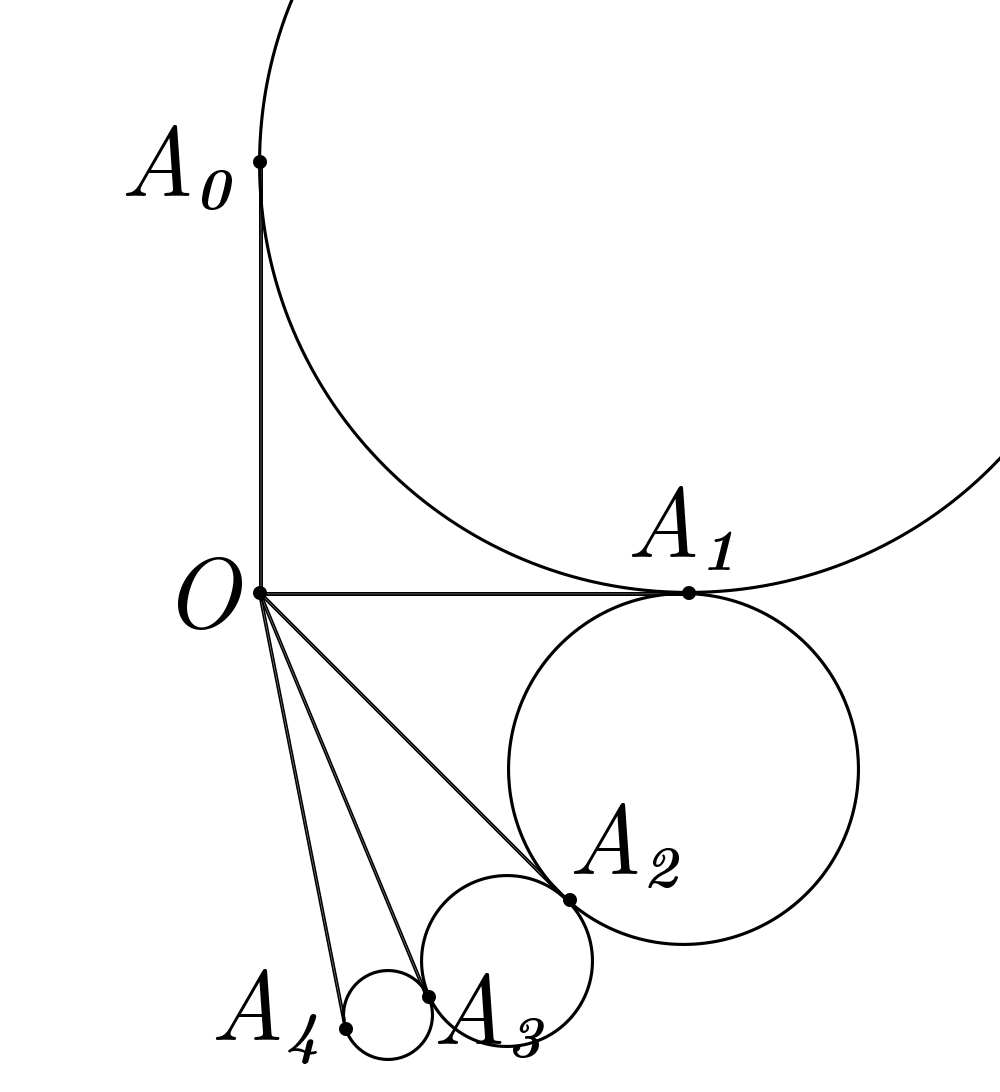
\includegraphics[width=\textwidth]{f2.png}
  \end{center}
\end{minipage}%
\begin{enumerate}[start=3]
  \item Two circles, both radius $\sqrt2$, have centers $\sqrt{3}-1$ apart. What is the area of their common region?

  \fourch
  {$\dfrac{5\pi}3 - 1$}
  {$2\pi - \dfrac12$}
  {$\dfrac{4\pi}3 - \dfrac12$}
  {$\dfrac{7\pi}3 - \dfrac{\sqrt3}2$}

  \item Four people are trying to guess the location of a point $X$ in the Cartesian plane. The guess closest to $X$ was $(1, 0)$, the second-closest was $\del{\frac32, \frac{\sqrt3}2}$, the third-closest was $(0, 0)$, and the farthest was $\del{\frac12, -\frac{\sqrt3}2}$. Given this information, what is the area of the region where point $X$ can be located?

  \fourch
  {$\dfrac{\sqrt3}8$}
  {$\dfrac{\sqrt3}6$}
  {$\dfrac{\sqrt3}4$}
  {$\dfrac{\sqrt3}3$}

  \item For a positive integer $n$, let $f(n) = -1$ if the sum of the exponents in its prime factorization is odd, and $f(n) = 1$ if it is even. For example, $f(1) = 1$, $f(5) = -1$, and $f(24) = f\del{2^3 \cdot 3} = 1$ since $3+1$ is even. What is the sum of $df(d)$ over all positive factors $d$ of $6480$?

  \fourch
  {$-22\,506$}
  {$-2684$}
  {$2684$}
  {$22\,506$}

  \item For how many integers $0 \leq k \leq 2017^2$ does $2017$ divide $\displaystyle \binom{2017^2}{k}$?

  \fourch
  {$2017^2-2017$}
  {$2017^2-2016$}
  {$2017^2-1$}
  {$2017^2$}

  \item Polynomial $P(x)$ has rational coefficients, degree $4032$, and leading coefficient $2017^2$. The numbers $\dfrac1{\sqrt2}, \dfrac1{\sqrt3}, \ldots, \dfrac1{\sqrt{2017}}$ are $2016$ of its roots. What is the sum of its coefficients?

  \fourch
  {$\dfrac{1}{2017}$}
  {$0$}
  {$1$}
  {$2017$}

  \item Evaluate the sum $$\frac{\log_{2^2} 1 - 1}{\log_{2^2} 2017 + \log_{2^2} 2017!} + \frac{\log_{3^2} 2 - 1}{\log_{3^2} 2017 + \log_{3^2} 2017!} + \cdots + \frac{\log_{2017^2} 2016 - 1}{\log_{2017^2} 2017 + \log_{2017^2} 2017!},$$ where the numerator is $\log_{n^2} (n-1) - 1$ and the denominator is $\log_{n^2} 2017 + \log_{n^2} 2017!$, the sum ranging from $n = 2$ to $2017$.

  \fourch
  {$-2$}
  {$-1$}
  {$0$}
  {$1$}

  \item Trapezoid $ABCD$ has $AB$ parallel to $CD$, $AB = 25$, $AC = 20$ and $AD = BC = 15$. Find its area.

  \fourch
  {$128$}
  {$144$}
  {$180$}
  {$192$}

  \item How many ways are there to tile a $3 \times 15$ rectangle with $3 \times 1$ and $1 \times 3$ tiles? Rotations and reflections are counted as different tilings.

  \fourch
  {$162$}
  {$171$}
  {$180$}
  {$189$}
\end{enumerate}

\vspace{1em}
\noindent\textbf{PART III.} All answers should be in simplest form. Each correct answer is worth six points.
\vspace{1em}

\noindent
\begin{minipage}{0.65\textwidth}
  \begin{enumerate}
    \item Chris has $2018$ matchsticks, and forms several digits with them, using the pattern shown in the figure on the right. What is the largest possible sum of the digits Chris can make?

    \item In triangle $ABC$, let $A_B$ and $A_C$ be the reflections of $A$ with respect to $B$ and $C$ respectively. Define $B_A, B_C, C_A$ and $C_B$ similarly. Find the ratio of the area of the hexagon $A_BA_CB_CB_AC_AC_B$ to the area of triangle $ABC$.

    \item What is the sum of the prime factors of $3\,200\,021$?
  \end{enumerate}
\end{minipage}%
\begin{minipage}{0.35\textwidth}
  \begin{center}
    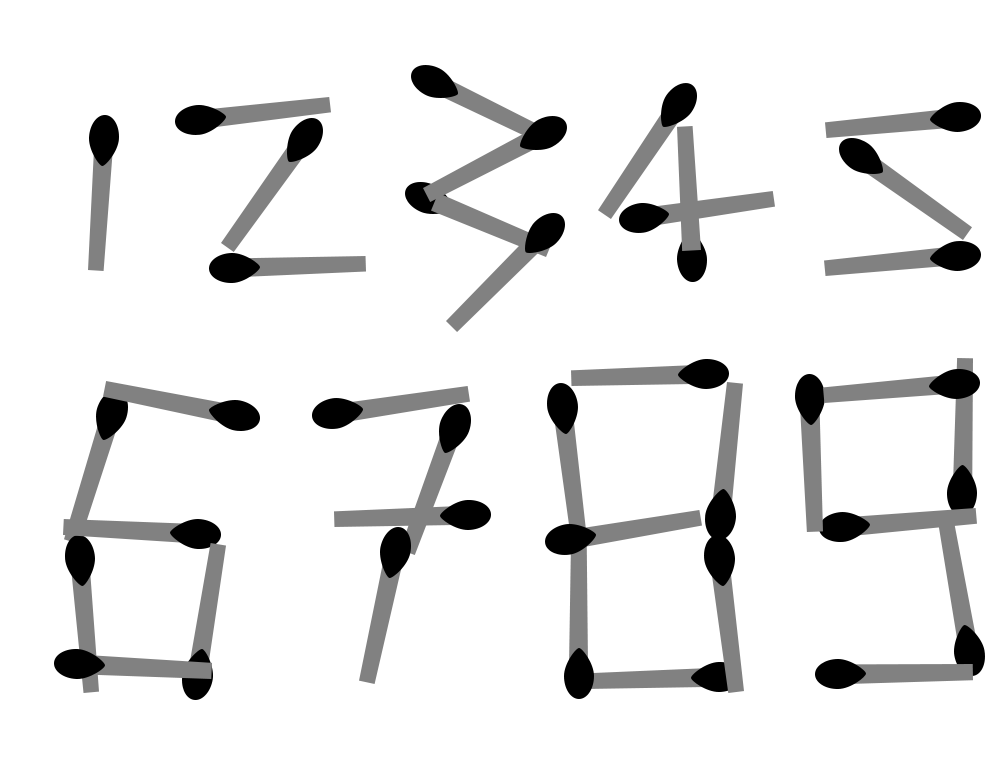
\includegraphics[width=0.9\textwidth]{f3.png}
  \end{center}
\end{minipage}

\begin{enumerate}[start=4]
  \item The function $f : \RR \to \RR$ satisfies $f(1) = 0$ and $$\frac{f(x+y)+f(x-y)}x - 4x^2 = \frac{f(x+y)-f(x-y)}y - 4y^2$$ for all nonzero $x$ and $y$. Find the value of $f(20) - f(17)$. 

  \item It is possible to write every positive integer uniquely as a \emph{proper sum} like so: $$8 = 1 + 1 + 2 + 4 \qquad 81 = 1 + 2 + 2 + 4 + 8 + 16 + 16 + 32 \qquad 15 = 1 + 2 + 4 + 8$$ A proper sum has consecutive powers of two, starting from $1$. Every power of two in a proper sum appears either once or twice. The following sums are \emph{not} proper: $$13 = 1 + 2 + 2 + 8 \qquad 10 = 2 + 4 + 4 \qquad 7 = 1 + 2 + 2 + 2$$ Let $f(n)$ be the number of powers of two that appear twice in the proper sum of $n$. For example, $f(81) = 2$, since $2$ and $16$ appear twice. Find the $70$th smallest positive integer $n$ with $f(n) = 3$.
\end{enumerate}

\end{document}
